%%Einleitung in das Thema der Arbeit

\chapter{Aktuelle Bedeutung der SaaS-Anwendungen}

Mit \textit{Software-as-a-Service} (SaaS) Anwendungen werden Programme bezeichnet, welche dem Kunden als Dienstleistung angeboten wird, jedoch auf der IT-Infrastruktur des Dienstleisters betrieben wird. Der Kunde kann also auf den Dienst zugreifen, ohne eine eigenen ausreichende Umgebung für dessen Betrieb zu besitzen. Meist erfolgt dieser Zugriff über Web-Schnittstellen \cite{McNee2007}. Durch die für den Kunden einfache Nutzung steigt der Bedarf nach der derartigen Angeboten.\\

So prognostiziert das Beratungsunternehmen Gartner, dass Produkte auf Basis von SaaS auch in den folgenden zwei Jahren deutlich mehr Umsatz generieren werden, wie in Abbildung \ref{fig:GartnerSaaS} zu sehen ist. 

\begin{figure}[h]
	\centering
	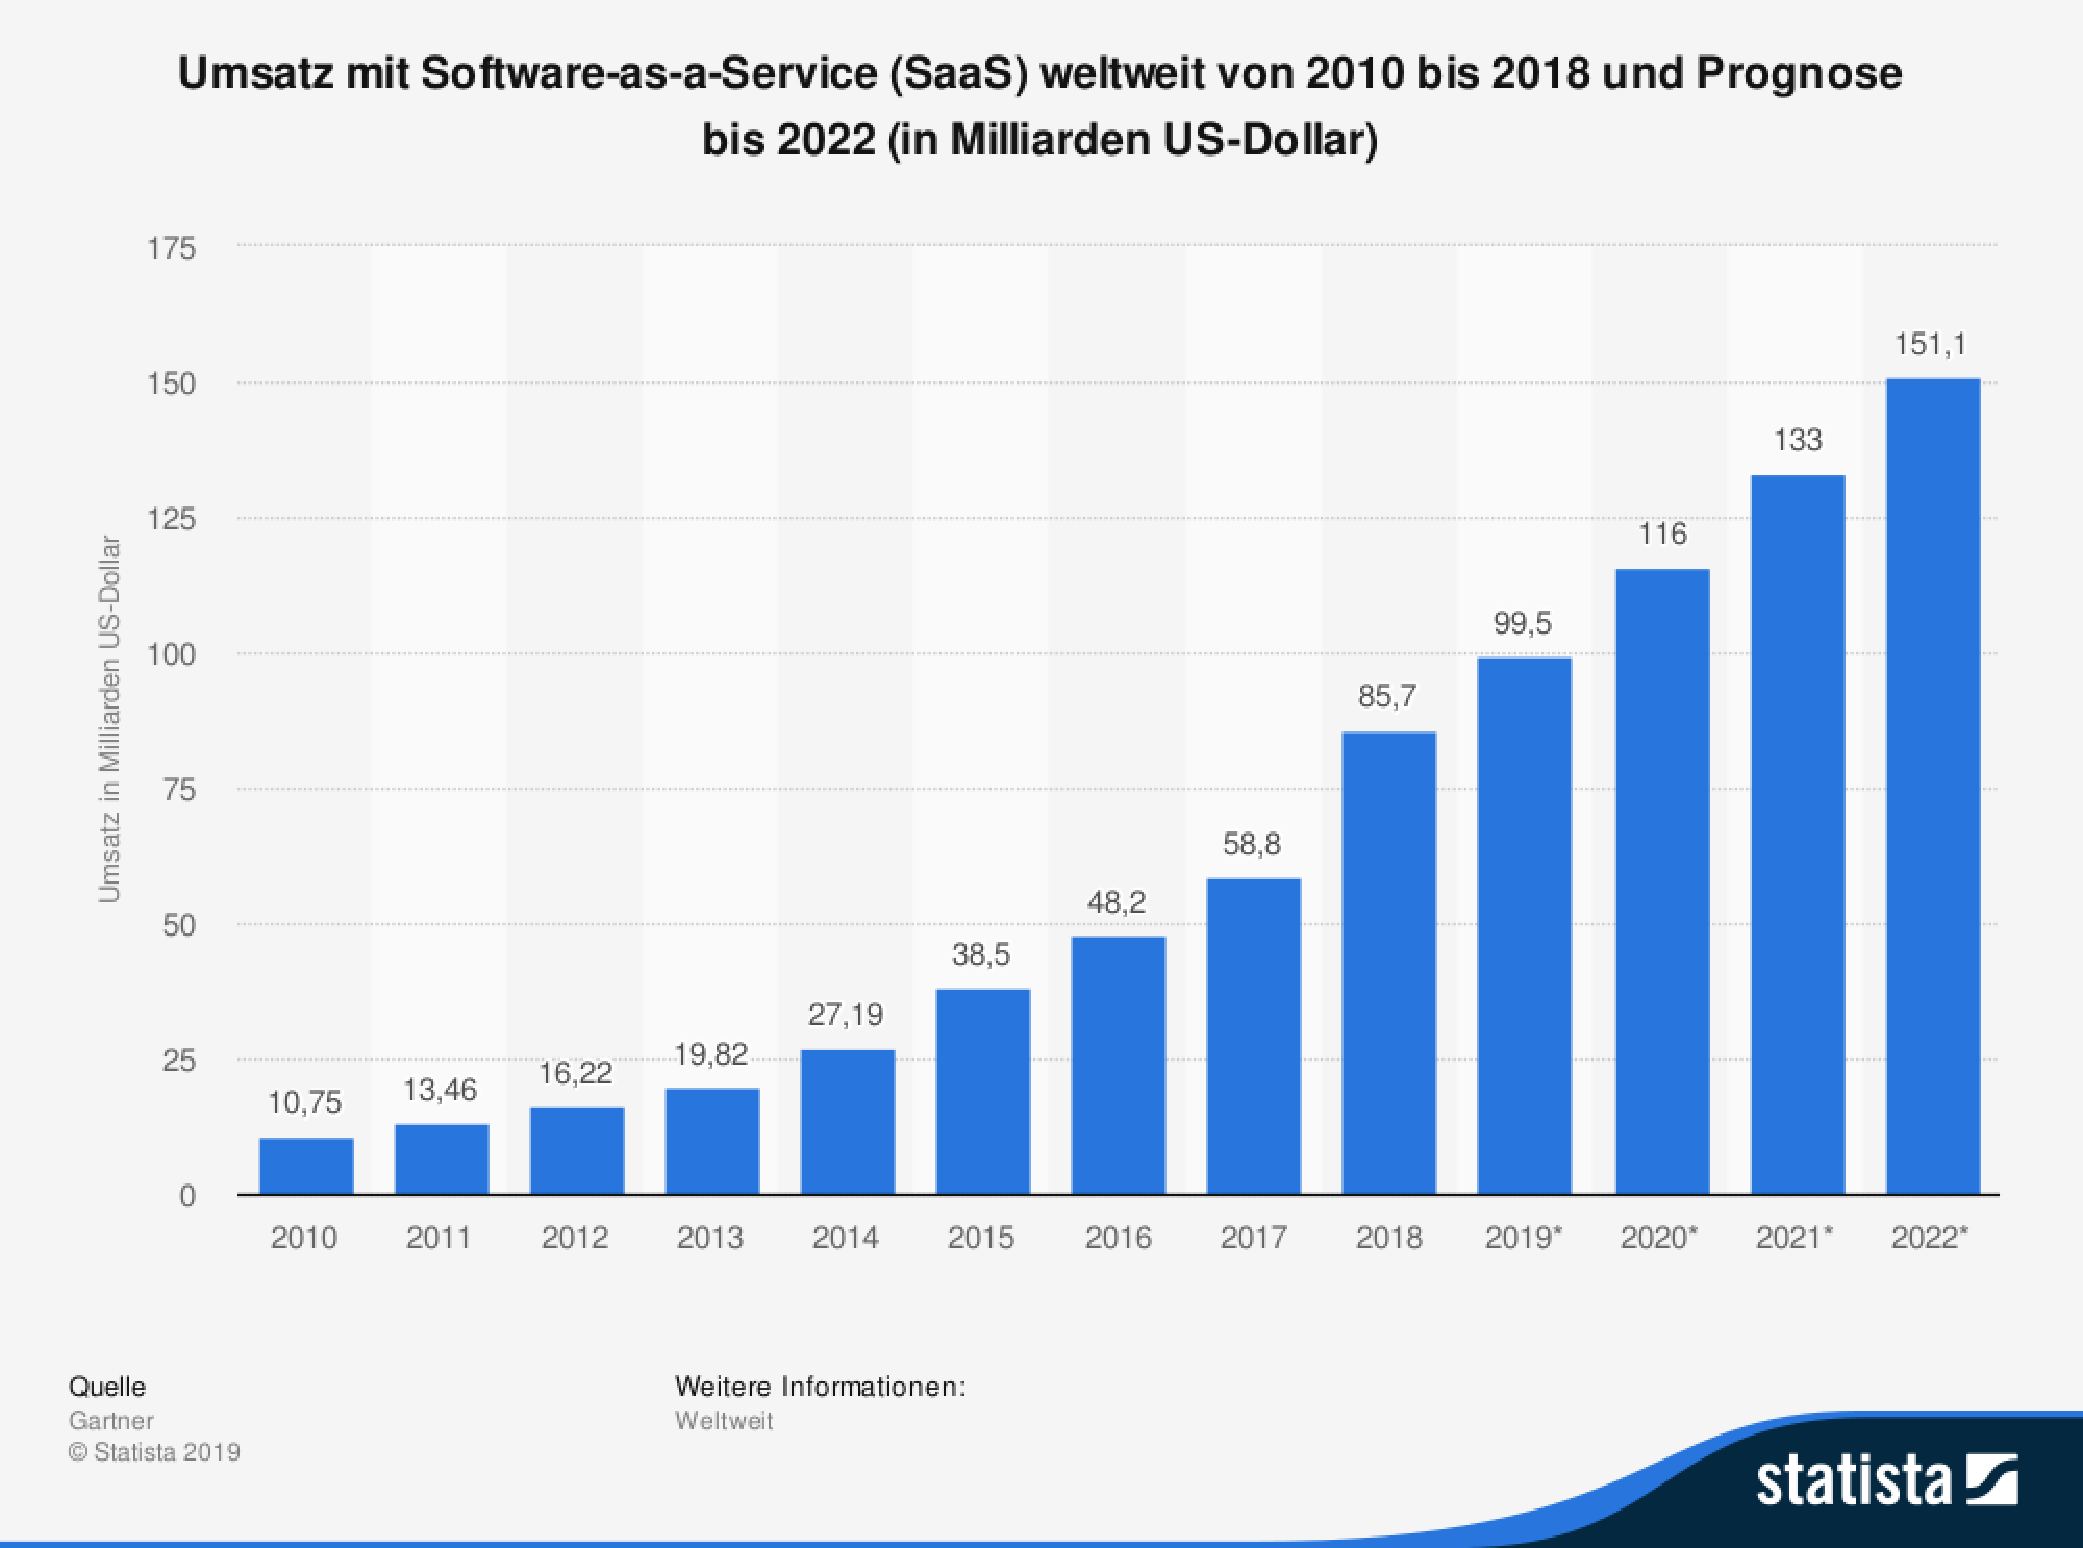
\includegraphics[width=1\textwidth]{Bilder/einleitung/SaaSUmsatzentwicklung}
	\caption{Prognose zum Umsatz mit \textit{Software-as-a-Service} Weltweit bis 2022 \cite{Gartner2020}}
	\label{fig:GartnerSaaS}
\end{figure}

SaaS-Anwendungen sind zudem der stärkste Umsatzzweig nach Gartner den Abstand zu den \textit{Infrastructure-as-a-Service} (IaaS) Anwendungen ausbauen, wie in Abbildung \ref{fig:GartnerSaaS2} zu sehen ist \cite{Gartner2019}.

\begin{figure}[h]
	\centering
	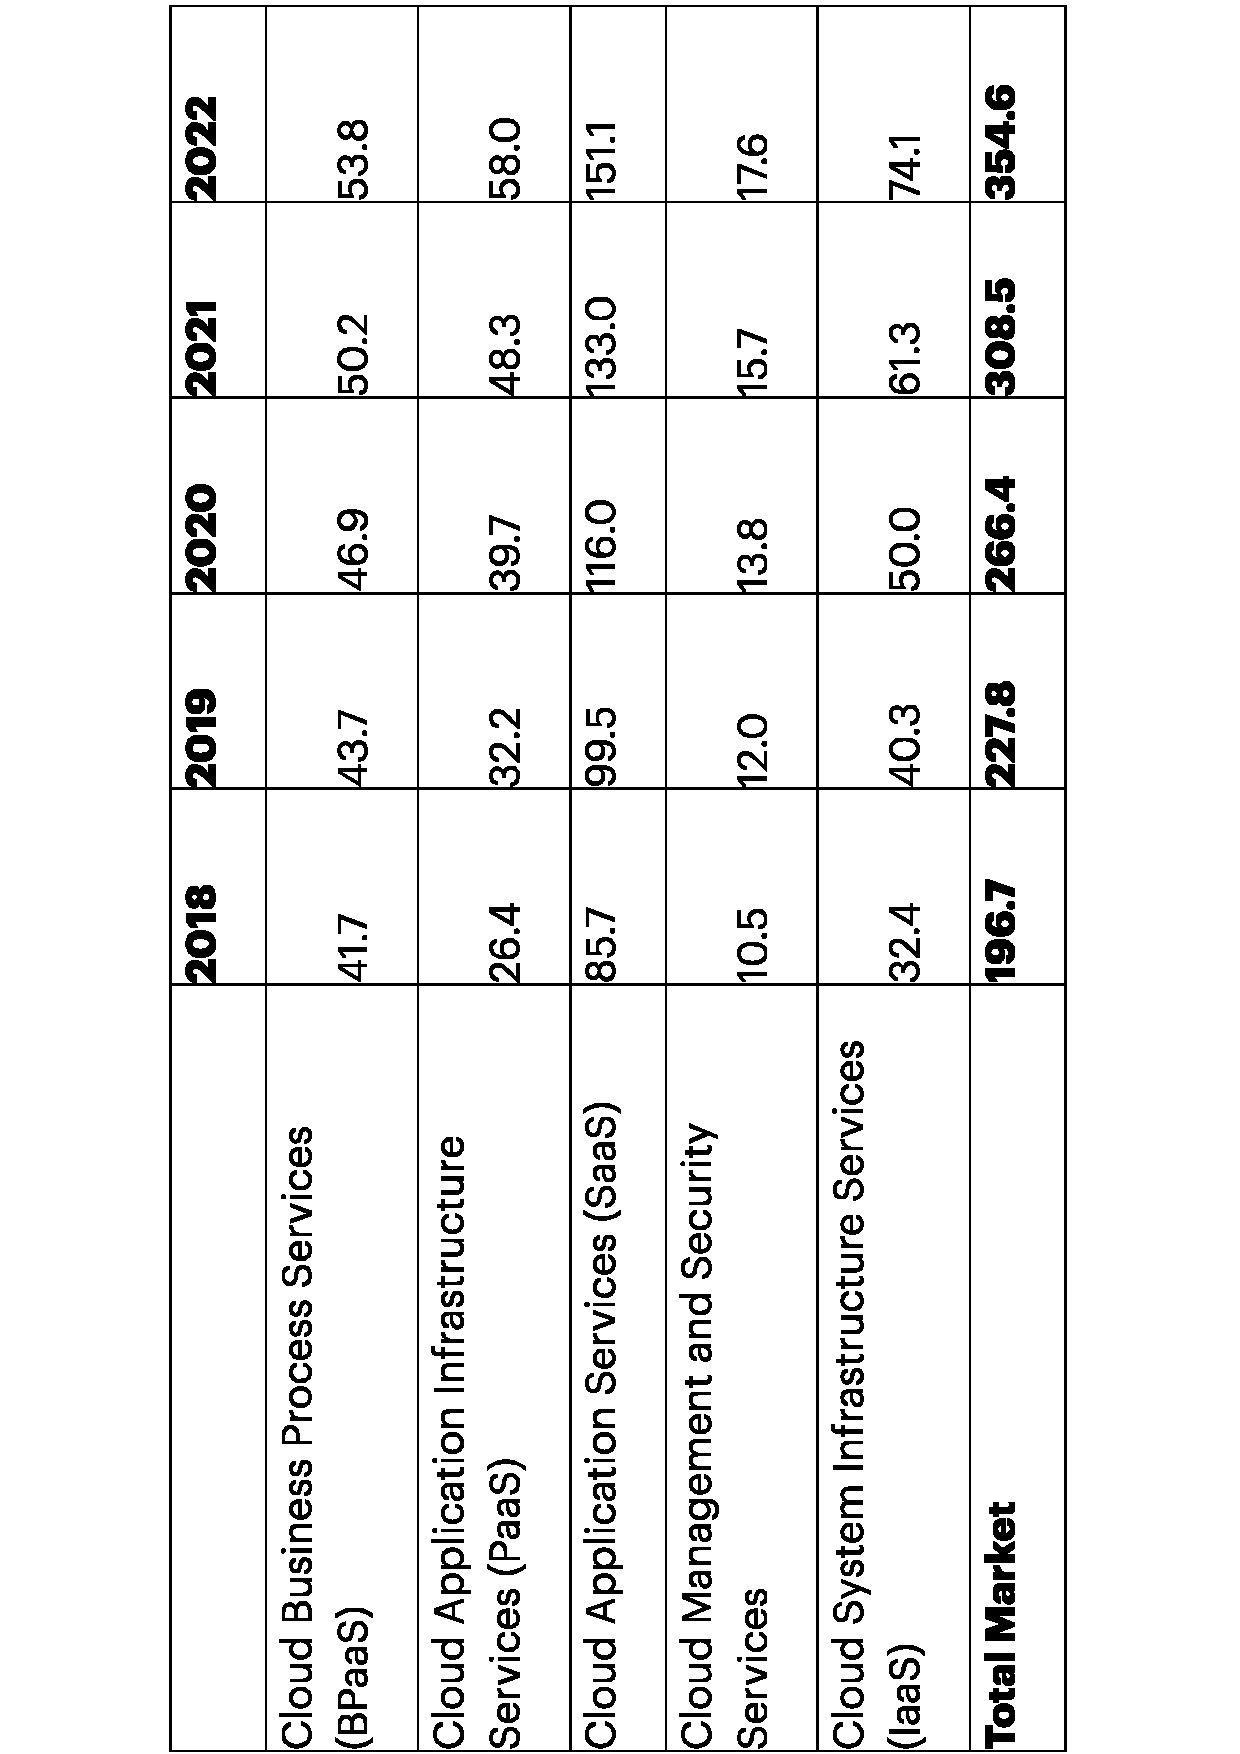
\includegraphics[angle=-90, width=1\textwidth]{Bilder/einleitung/Gartner1}
	\caption{Weltweite Prognose des Umsatzes mit öffentlichen \textit{Cloud}-Diensten \cite{Gartner2019}}
	\label{fig:GartnerSaaS2}
\end{figure}

Da allerdings eine Vielzahl an Diensten vorhanden ist, sind die Daten oft zwischen diesen verteilt. Möchte nun ein Kunde das Angebot wechseln und stellt der neue Anbieter keine Konvertierungsmöglichkeit für die Daten des anderen Anbieters bereit, so muss der Kunde entweder die Daten selbstständig übertragen oder auf diese verzichten. Dieses Problem kann jedoch durch Extrahierung in Injektion der Informationen durch die gegebenen Anwendungsschnittstellen und eine externe Konvertierung in einem neuen Anwendungsprogramm behoben werden. Für die Erstellung eine Prototypen wird ein Projekt mit Simon Hofmeister und Stephan Nunhofer unter der Aufsicht von Prof. Dr. Johannes Schildgen gestartet.